\begin{frame}{Teachers}
%  Lecturers:
%  \begin{
%  \begin{itemize}
%    \item Patrick Forr\'e, \url{p.d.forre@uva.nl}
%      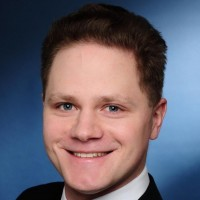
\includegraphics[width=3cm]{PatrickForre.jpg}
%    \item Joris Mooij, \url{j.m.mooij@uva.nl}
%      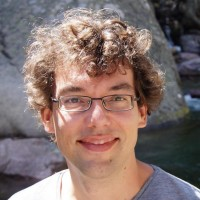
\includegraphics[width=3cm]{JorisMooij.jpg}
%  \end{itemize}
%
%  \bigskip
%  Teaching Assistants:
%  \begin{itemize}
%    \item Noud de Kroon, \url{a.a.w.m.dekroon@uva.nl}
%      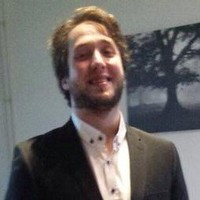
\includegraphics[width=3cm]{NoudDeKroon.jpg}
%    \item Philip Boeken, \url{p.boeken@uva.nl}
%      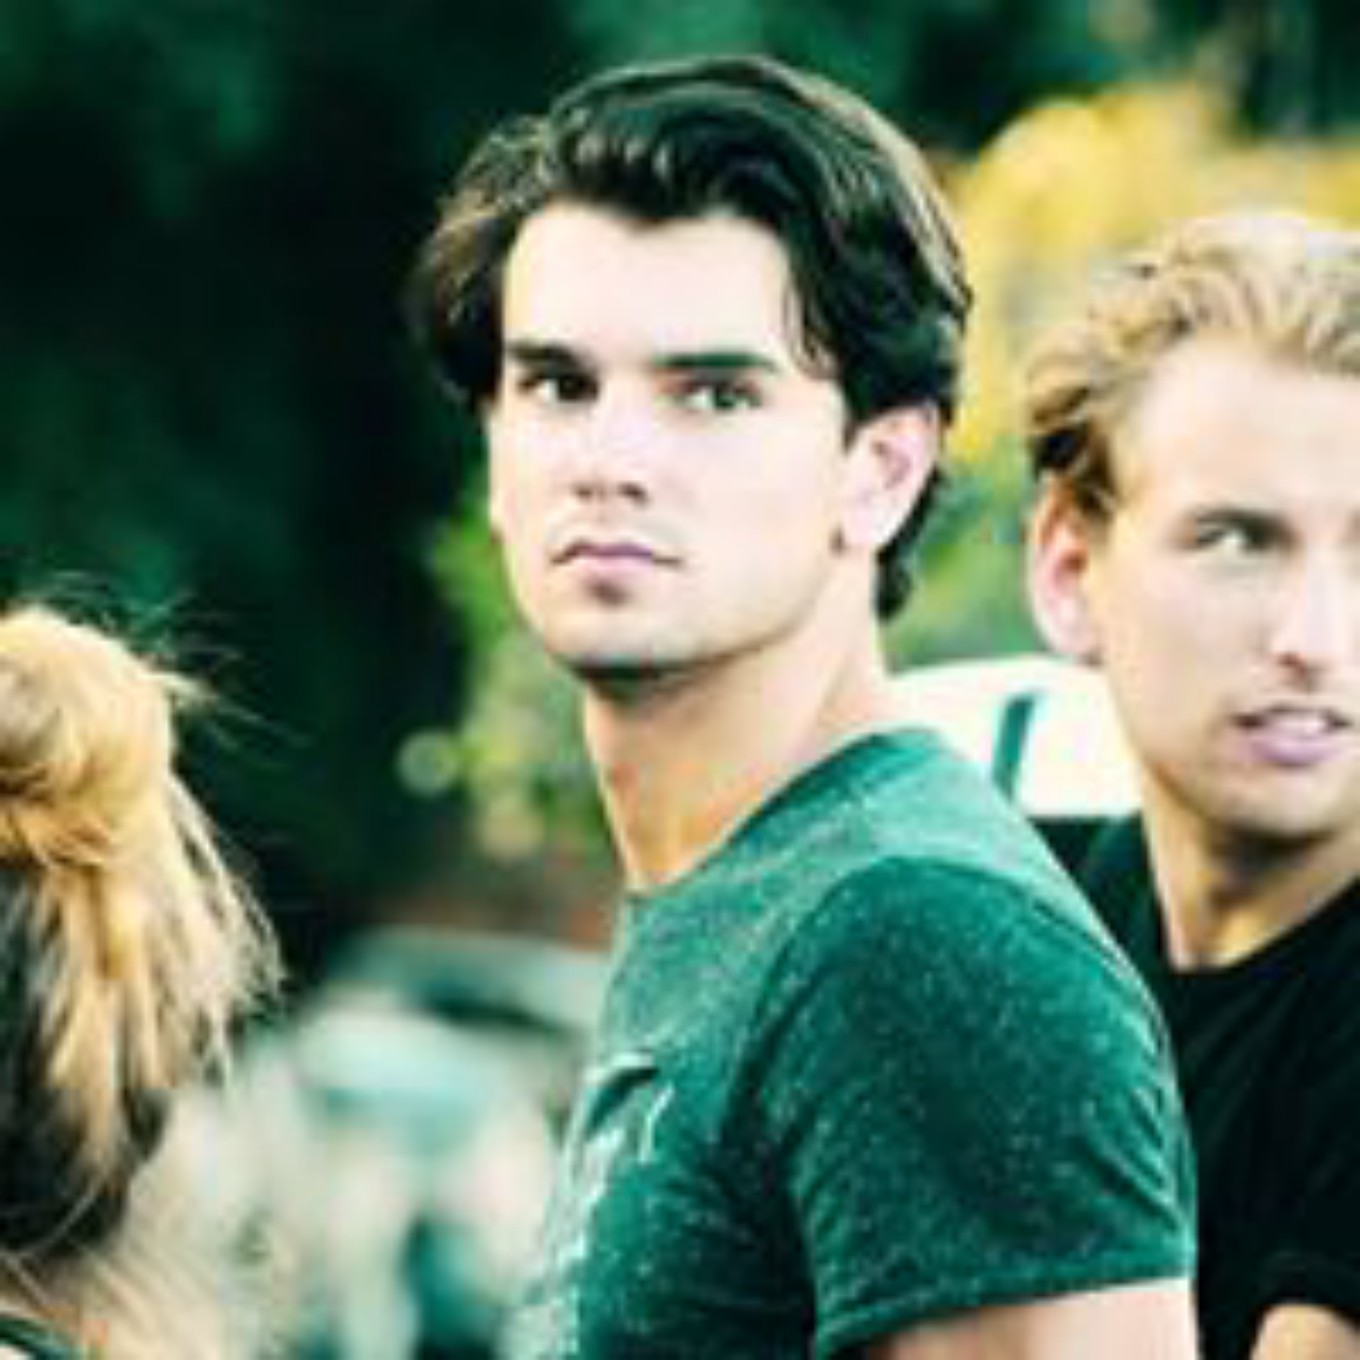
\includegraphics[width=3cm]{PhilipBoeken.jpg}
%  \end{itemize}

  Lecturers:\\
  \scalebox{1.00}{\begin{tikzpicture}
      \node at (-4,0) {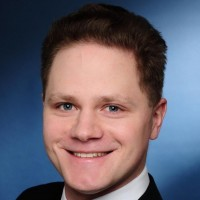
\includegraphics[height=2cm]{PatrickForre.jpg}};
      \node at (-4,-1.5) {Patrick Forr\'e};
      \node at (-4,-2) {\footnotesize \url{p.d.forre@uva.nl}};
      \node at (0,0) {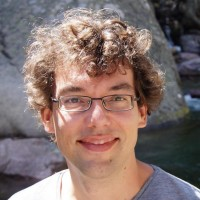
\includegraphics[height=2cm]{JorisMooij.jpg}};
      \node at (0,-1.5) {Joris Mooij};
      \node at (0,-2) {\url{j.m.mooij@uva.nl}};
  \end{tikzpicture}}

  \bigskip
  Teaching assistants:\\
  \begin{tikzpicture}
      \node at (-4,0) {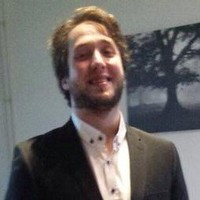
\includegraphics[height=2cm]{NoudDeKroon.jpg}};
      \node at (-4,-1.5) {Noud de Kroon};
      \node at (-4,-2) {\footnotesize \url{a.a.w.m.dekroon@uva.nl}};
      \node at (0,0) {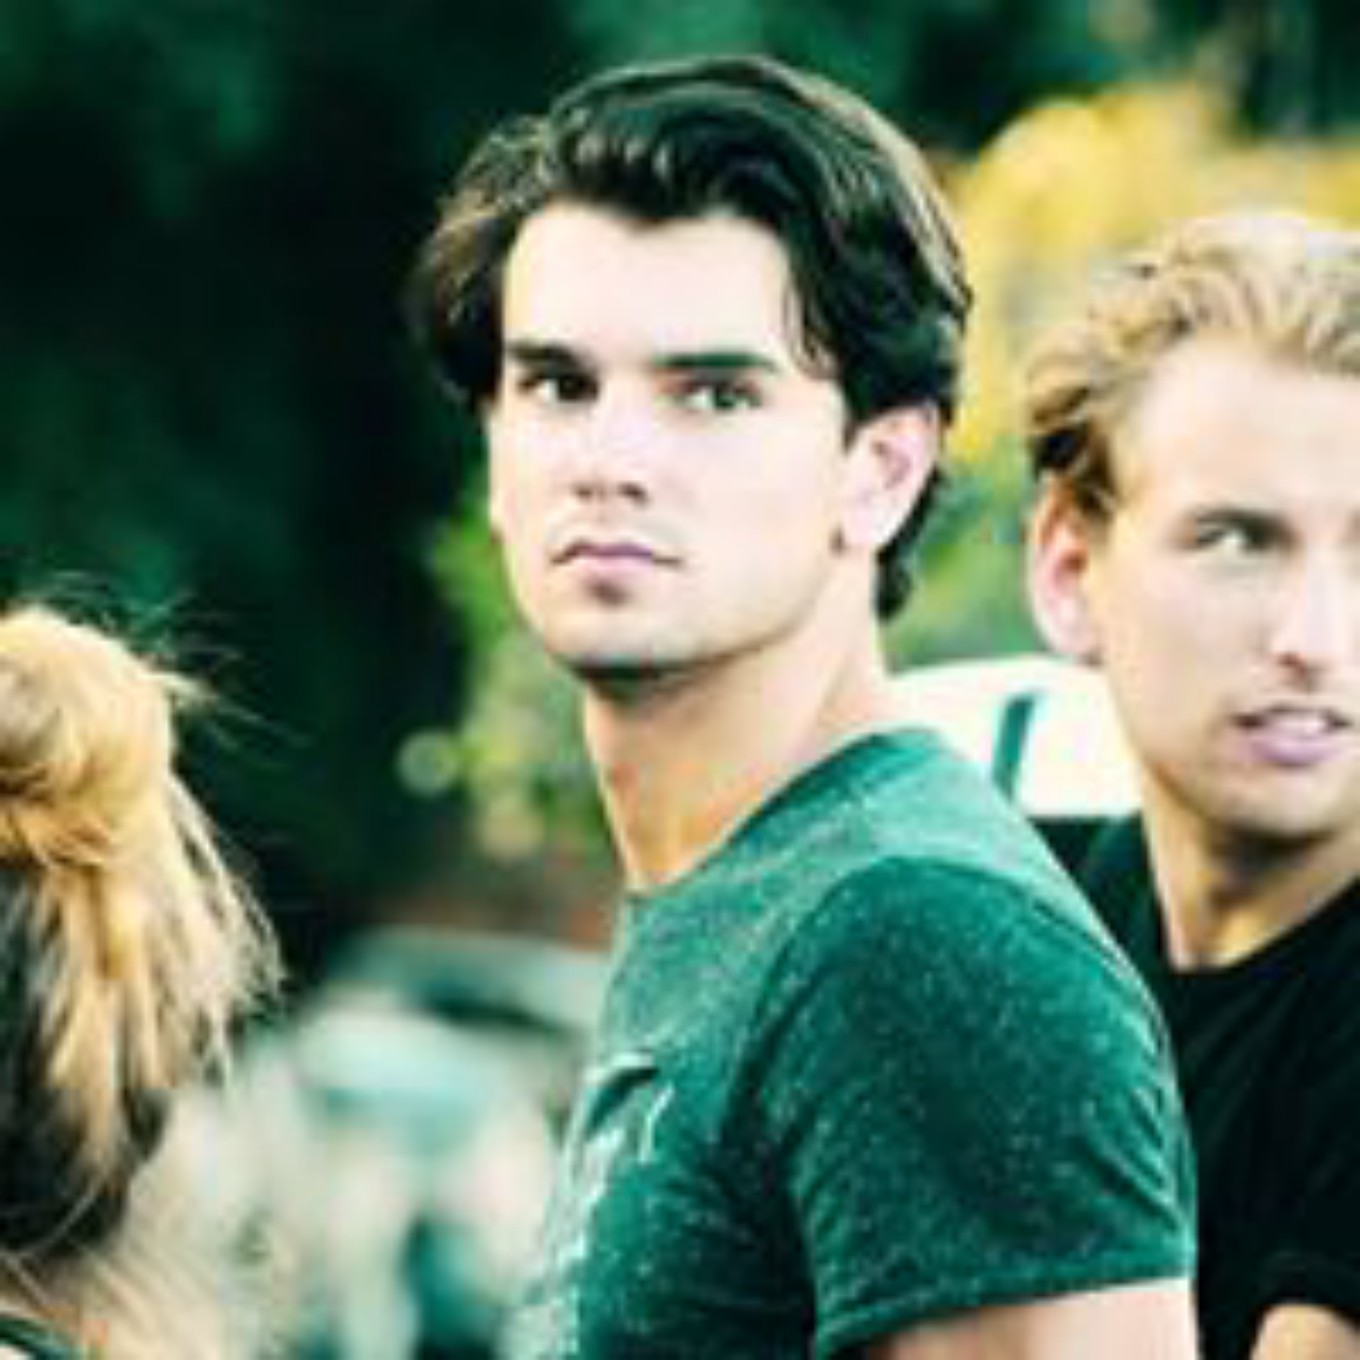
\includegraphics[height=2cm]{PhilipBoeken.jpg}};
      \node at (0,-1.5) {Philip Boeken};
      \node at (0,-2) {\footnotesize \url{p.a.boeken@uva.nl}};
  \end{tikzpicture}
\end{frame}

\begin{frame}{Target Audience}
  Designed for:
  \begin{itemize}
    \item MSc.\ Mathematics
    \item MSc.\ Stochastics \& Financial Mathematics
  \end{itemize}
  students with Measure Theoretic Probability as a prerequisite.

  \bigskip
  We also welcome:
  \begin{itemize}
    \item MSc.\ AI students
    \item students from other MSc. programs
    \item PhD students
  \end{itemize}
  BUT: hard work required to compensate for mathematical deficits, in particular to acquire \textbf{passive understanding of measure theoric formulations}.
  
  \bigskip
  (Bonus: measure theory is the \textit{lingua franca} of probability theory and statistics)
\end{frame}

\begin{frame}{Course materials}
  \begin{itemize}
    \item Canvas page
    \item Live lectures
    \item Lecture notes (weekly chunks and as complete work-in-progress)
    \item Weekly exercises
    \item Video lectures from last year (as backup in case of illness etc.)
  \end{itemize}
\end{frame}

\begin{frame}{Timeline}
  \begin{itemize}
    \item Weeks 1-7: Patrick will teach Markov kernels and Causal Bayesian Networks
    \item Weeks 9-16: Joris will teach Structural Causal Models and causal discovery
    \item Breaks in weeks 8, 11, 13
    \item Exam in week 17
  \end{itemize}
\end{frame}

\begin{frame}{Exercises, grading}
  Weekly exercises:
  \begin{itemize}
    \item Two groups, scheduled sequentially
    \item Check whether current group assignment matches your schedule (if not, email me)!
    \item Will be graded.
  \end{itemize}

  \bigskip
  Final degree will consist of
  \begin{itemize}
    \item 15\% exercises
    \item 85\% exam
  \end{itemize}
\end{frame}

\begin{frame}{Questions?}
  Any questions so far?
\end{frame}
